%%%%%%%%%%%%%%%%%%%%%%%%%%%%%%%%%%%%%%%%%%%%%%%%%%%%%%%%%%%%%%%%%%%%%%%%%%%%%%%%%%%%%%%%%%%%%%%%%%%%%%%%%%%%%%%%%%%%%%%%%%%%%%%%%%%%%%%%%%%%%%%%%%%%%%%%%%%
% This is just an example/guide for you to refer to when submitting manuscripts to Frontiers, it is not mandatory to use Frontiers .cls files nor frontiers.tex  %
% This will only generate the Manuscript, the final article will be typeset by Frontiers after acceptance.   
%                                              %
%                                                                                                                                                         %
% When submitting your files, remember to upload this *tex file, the pdf generated with it, the *bib file (if bibliography is not within the *tex) and all the figures.
%%%%%%%%%%%%%%%%%%%%%%%%%%%%%%%%%%%%%%%%%%%%%%%%%%%%%%%%%%%%%%%%%%%%%%%%%%%%%%%%%%%%%%%%%%%%%%%%%%%%%%%%%%%%%%%%%%%%%%%%%%%%%%%%%%%%%%%%%%%%%%%%%%%%%%%%%%%

%%% Version 3.4 Generated 2018/06/15 %%%
%%% You will need to have the following packages installed: datetime, fmtcount, etoolbox, fcprefix, which are normally inlcuded in WinEdt. %%%
%%% In http://www.ctan.org/ you can find the packages and how to install them, if necessary. %%%
%%%  NB logo1.jpg is required in the path in order to correctly compile front page header %%%

\documentclass[utf8]{template/frontiersSCNS} % for Science, Engineering and Humanities and Social Sciences articles
%\documentclass[utf8]{frontiersHLTH} % for Health articles
%\documentclass[utf8]{frontiersFPHY} % for Physics and Applied Mathematics and Statistics articles

%\setcitestyle{square} % for Physics and Applied Mathematics and Statistics articles
% \usepackage{url,hyperref,lineno,microtype,subcaption}
\usepackage{url,hyperref,lineno,microtype}
\usepackage[onehalfspacing]{setspace}

% \linenumbers # commented out when sending the abstract

% Leave a blank line between paragraphs instead of using \\

\def\keyFont{\fontsize{8}{11}\helveticabold }
\def\firstAuthorLast{Nalborczyk {et~al.}} %use et al only if is more than 1 author
\def\Authors{Ladislas Nalborczyk\,$^{1,2,*}$, Ursula Debarnot\,$^{3,4}$, Marieke Longcamp\,$^{2}$, Aymeric Guillot\,$^{3,4}$, and F.-Xavier Alario\,$^{1}$}
% Affiliations should be keyed to the author's name with superscript numbers and be listed as follows: Laboratory, Institute, Department, Organization, City, State abbreviation (USA, Canada, Australia), and Country (without detailed address information such as city zip codes or street names).
% If one of the authors has a change of address, list the new address below the correspondence details using a superscript symbol and use the same symbol to indicate the author in the author list.
\def\Address{$^{1}$Aix Marseille Univ, CNRS, LPC, Marseille, France \\
$^{2}$Aix Marseille Univ, CNRS, LNC, Marseille, France \\
$^{3}$Inter-University Laboratory of Human Movement Biology-EA 7424, University of Lyon, University Claude Bernard Lyon 1, Villeurbanne, France \\
$^{4}$Institut Universitaire de France, Paris, France}
% The Corresponding Author should be marked with an asterisk
% Provide the exact contact address (this time including street name and city zip code) and email of the corresponding author
\def\corrAuthor{Corresponding Author}
\def\corrEmail{ladislas.nalborczyk@univ-amu.fr}

\begin{document}
\onecolumn
\firstpage{1}

\title[Covert verbal actions]{What covert verbal actions tell us about the interplay between language, action, and perception}

\author[\firstAuthorLast ]{\Authors} %This field will be automatically populated
\address{} %This field will be automatically populated
\correspondance{} %This field will be automatically populated

\extraAuth{}% If there are more than 1 corresponding author, comment this line and uncomment the next one.
%\extraAuth{corresponding Author2 \\ Laboratory X2, Institute X2, Department X2, Organization X2, Street X2, City X2 , State XX2 (only USA, Canada and Australia), Zip Code2, X2 Country X2, email2@uni2.edu}

\maketitle

\begin{abstract}

\noindent Humans have a remarkable ability to imagine actions without executing them. Such motor imagery is accompanied by a subjective multisensory experience with auditory, visual, and kinaesthetic components. An influential hypothesis states that these sensory percepts result from a simulation of the corresponding motor action that relies on the same internal models recruited for the control of overt actions. A significant consequence of this hypothesis is that the sensory experience of covert actions would be continuously shaped by sensorimotor interactions with the environment. However, the precise computations required by these internal models and their neural implementation remain unclear. Moreover, this simulationnist view raises the question of how it is possible to imagine actions without executing them. In this perspective, we focus on covert verbal actions such as covert speech, writing, or typing, as an exciting case study to help understanding the interplay between language, motor control, and perceptual processes. 

% Since the first explorations of the phenomenological and psychophysiological properties of imagined actions, there has been considerable efforts and progresses towards describing the mechanisms leading to these sensory percepts.

\tiny
 \keyFont{\section{Keywords:} motor imagery, motor simulation, motor control, response inhibition, covert speech} % All article types: you may provide up to 8 keywords; at least 5 are mandatory.
\end{abstract}

\newpage

\section{Introduction}

%%%%%%%%%%%%%%%%%%%%%%%%%%%%%%%%%%%%%%%%%%%%%%%%
% Succinct introduction in four paragraphs.
% ------------------------------------------
% 1) Introduction of motor imagery
% 2) Covert verbals actions
% 3) Relating 1) and 2) to the thematic of the research topic
% 4) Aims of the present perspective
%%%%%%%%%%%%%%%%%%%%%%%%%%%%%%%%%%%%%%%%%%%%%%%

The ability to mentally examine our thoughts is central to our subjective experience. Mentally anticipating or rehearsing (verbal) actions allows us to become better at performing them \citep[e.g.,][]{toth2020}, to explore/practise novel situations \citep{babar}, or to rehearse past situations \citep{babar}. Broadly construed, motor imagery can be defined as the mental process by which one rehearses an action without engaging in the physical movements involved in this particular action. Because speech production results from sequences of motor commands that are assembled to reach a given communication goal, it belongs to the broader category of motor actions \citep{jeannerod_motor_2006}. Therefore, a parallel can be drawn between covert speech (also known as \textit{inner speech} or \textit{speech imagery}) \citep[for reviews, see][]{alderson-day_inner_2015, perrone-bertolotti_what_2014, loevenbruck_cognitive_2018} and other forms of covert verbal actions such as covert signing, covert writing, or covert typing and, more generally, other imagined actions.

% One of the most influential theoretical model of motor imagery the motor simulation theory \cite{jeannerod_origin_2006, jeannerod_representing_1994, jeannerod_neural_2001}, postulates the existence of a continuum between the covert and the overt execution of an action and that action representations can operate off-line via a simulation mechanism. In short, covert actions would rely on the same set of mechanisms as the overt actions they simulate, except that execution is inhibited \citep{oshea_does_2017}. A second class of models are concerned with the phenomenon of emulation \citep{grush_emulation_2004} and with internal models \cite[for a review of the similarities and dissimilarities between simulation and emulation models, see][]{gentsch_towards_2016}. Internal model theories share the postulate that action control uses internal models, that is, systems that simulate the behaviour of the motor apparatus \citep[e.g.,][]{jordan_forward_1992, kawato_hierarchical_1987}. The function of internal models is to estimate and anticipate the outcome of a motor command. Among the internal model theories, motor control models based on robotic principles \citep[e.g.,][]{kawato_internal_1999, wolpert_internal_1995} assume two kinds of internal models: a forward model (or simulator) that predicts the sensory consequences of motor commands from efference copies of the issued motor commands, and an inverse model (or controller) that calculates the feedforward motor commands from the desired sensory states \citep{gentsch_towards_2016, loevenbruck_cognitive_2018}. Notice that in the following, we do not distinguish further between simulation and emulation, and we use these terms interchangeably to designate the mechanism through which sensory consequences of motor commands (or copy thereof) are computed by forward internal models.

% By building upon models of speech motor control (e.g., Houde \& Nagarajan, 2011; Wolpert et al., 1995), a recent model describes wilful (voluntary) expanded covert speech as "multi-modal acts with multi-sensory percepts stemming from coarse multi-sensory goals" \cite{loevenbruck_cognitive_2018}. In other words, this model considers the auditory and kinaesthetic sensations perceived during covert speech to be the predicted sensory consequences of inhibited speech motor acts, emulated by internal forward models that use the efference copies issued from an inverse model (this proposal shares some similarities with the emulation model of motor imagery, Grush, 2004) \cite{grush_emulation_2004}. This model is supported by several empirical results providing both behavioural and neurophysiological evidence for the efference copies issued during inner speech production (e.g., Scott, 2013; Whitford et al., 2017)...

In this perspective, we examine some theoretical and experimental consequences of considering covert verbal actions as other forms of imagined actions. We explore two main themes. First, we discuss the plausible origins of the multisensory (e.g., auditory, kinaesthetic) content of covert verbal actions. Second, we discuss the under-explored role of inhibitory mechanisms during motor imagery and covert verbal actions more specifically. By bridging together recent results from the motor imagery, motor inhibition, and covert speech literature, we highlight some novel and possibly fruitful lines of research.

\section{The interplay between motor control and cognition}

Where does the sensory content of covert verbal actions come from? How does motor learning shape these sensory percepts? In other words, how do the motor and perceptual system interact during covert verbal actions? In the first subsection, we discuss two mechanisms that may be responsible for providing the sensory content of covert verbal actions and their respective involvement in different forms of covert speech. In the second subsection, we discuss an exciting avenue for investigating the influence of motor learning on the sensory content of covert verbal actions, namely, the imagery of totally novel (i.e., never executed) verbal actions.

\subsection{Where does this sensory content come from?}

The production of covert speech is often (although not always and not for everyone) accompanied by the feeling of hearing speech \cite{hurlburt_investigating_2011}. In other words, covert speech is accompanied by a sensory experience that "feels like" hearing speech. In this section, we discuss the dual stream prediction model \citep{tian_mental_2012, tian_effect_2013, tian_mental_2016}, a theoretical account of the mechanisms leading to the generation of such auditory percepts during covert speech, while noticing that these mechanisms could be extended to other covert verbal actions as well.

The dual stream prediction model \citep{tian_mental_2012, tian_effect_2013, tian_mental_2016}... Direct simulation (attention-guided memory retrieval process) or indirect simulation (motor simulation process) \citep{tian_mental_2012, tian_effect_2013, li_corollary_2020, ma_distinct_2019}? The dual stream prediction model \citep{tian_mental_2016}... \citep[this proposal shares similarities with the distinction between the prediction-by-simulation or prediction-by-association mechanisms of][]{pickering_integrated_2013}.

The balance between these two mechanisms may depend on the precise instructions given to the participants, which may clue them to produce different form of covert speech. For instance, depending on whether participants are instructed to "imagine speaking" or to "imagine hearing" speech \citep[see also the distinction between the "inner ear" and the "inner voice", e.g.,][]{smith_subvocalization_1992}... Congruent with this hypothesis, it has been shown that inner speaking and inner hearing have distinct MEG correlates and effects on a subsequent /ba/-/ta/ categorisation task \citep{ma_distinct_2019}. Moreover...

In the absence of non-ambiguous instructions, and in line with \cite{tian_mental_2012}, we suggest that the balance between these two mechanisms may also depend on situational (e.g., surrounding noise) and intrinsic (e.g., expertise) characteristics. For instance... In addition to \cite{tian_mental_2012}, we suggest that a common currency determining the use of one of these mechanisms is the computational cost of (or equivalently, the computational resources available for) each alternative. To clarify, we borrow the concept of memoisation as applied to cognition and mental imagery by \cite{dasgupta_memory_2021}.\footnote{Memoisation is a programming technique used to speed-up algorithms or programs. It avoids redundant computation by storing computational results and reusing them later. When calling a function (where a function can be a motor primitive such as elevating the arm), the function call is intercepted by a memoiser that inspects the previous calls of a function and its outputs. If a function has already been called with the same input, then the previously computed output is retrieved and reused.} In this context, memory can be considered as a mechanism to facilitate computational reuse. In the same way efficient programming may rely on computational reuse, efficient cognition may rely on stored past computation results rather than reinventing the wheel every time. In the context of motor and speech imagery, the memory-retrieval predictions stream would be the memoised version of the simulation-estimation prediction stream, where motor-to-sensory mappings are (party or completely) retrieved from memory, instead of being computed again...

In other words, situational (extrinsic) and individual (intrinsic) characteristics jointly determine the computational cost (or equivalently, the available computational resources), which in turn determines the balance between the simulation and association mechanisms. For instance, we hypothesise that novel and/or difficult tasks (which are both computationally more expensive, ceteris paribus) may rely more on the simulation mechanism, whereas well known and/or easy tasks may rely more on associative mechanisms. This idea is supported by several studies showing a greater increase in facial EMG activity during the reading of difficult text or while performing difficult mental arithmetic tasks as compared to easier tasks \citep[e.g.,][]{faaborg-andersen_electromyography_1958, sokolov_inner_1972}, suggesting a greater involvement of the speech motor system \citep[and/or a lesser involvement of inhibitory mechanisms, see also the discussion in][]{nalborczyk_understanding_2019-1, nalborczyk_re-analysing_2020}. This is consistent with results from training studies suggesting that we rely more and more on domain-general (e.g., memory-based) processes with expertise \citep[e.g.,][]{tarr_mental_1989, jolicoeur_time_1985}.

% Memoisation: avoid redundant computation by storing computational results and reusing them later... functions call are intercepted with by a memoiser the inspects the previous calls of a function and its outputs. If a function has already been called with the same input, then the previously computed output is retrieved and reused... memoisation can be made more flexible (generalisable) by using \textit{interpolation} between cached outputs... for instance, in the context of motor control, reaching a goal (e.g., a cup of tea) can be decomposed in motor primitives, where input-output mapping can be retrieved from a memo table and/or interpolated from sufficiently similar stored mappings... or as put by \cite{dasgupta_memory_2021}, the "shift from algorithm to memory"... this shift is consistent with studies showing a lesser involvement of the motor system for well known imagined actions... Depending on whether the task needs to form "precise" sensory representations and whether we have the time resources to do it... Training studies also suggest that we rely more and more on domain-general (e.g., memory-based) processes with expertise \citep[e.g.,][]{tarr_mental_1989, jolicoeur_time_1985}.

\subsection{The motor imagery of novel actions}

If, as suggested in the previous section, the sensory content of covert verbal actions is (at least in some situations) provided by a motor simulation process, how can we imagine totally novel (i.e., never executed) actions? Broadly speaking, the simulationnist framework suggests that the multisensory experience of motor imagery results from the simulation of the corresponding motor action, reusing internal models developed for the control of overt actions. In other words, internal models developed for the control of actions would then be used to simulate the sensory consequences of covert actions. Crucially, these internal models are generative models, which means that they can be used to compute (i.e., predict) the sensory consequences of any action that can be parsed as a (possibly supramodal) goal to an inverse internal model. In other words, this framework makes it possible for novel actions to be simulated internally.\footnote{\cite{mulder_role_2004} assessed whether the mental practice of a totally novel movement (abduction of the big toe of the dominant right foot) resulted in better overt execution over the course of several weeks of practice. They observed that although mental practise did improve execution in the group of participants that already had some experience with the task at baseline, mental practise did not lead to statistically significant improvements in execution in the group of participants that had zero experience with the task at baseline. However, a Bayesian reanalysis of their results suggests that the evidence in favour of the null hypothesis was rather inconclusive ($\text{BF}_{01} = 1.92$, using a weakly informative Cauchy prior on the standardised effect size for the alternative hypothesis, with $r = 1$).}

A prediction of this putative mechanism is that the imagination of novel actions, and more precisely, the predicted sensory consequences of novel actions, may be "biased" or "constrained" by the repertoire of already-known actions. For instance, when asked to imagine playing table tennis, a tennis player may overestimate movements' amplitude and duration. Translated to speech production, this prediction could be assessed by asking participants to imagine a novel action and subsequently checking whether this improves the execution of an intermediate (interpolated) novel action in the articulatory space. The same logic could be applied to the covert production of speech with someone else's voice. How can we imagine speaking with the voice of our relatives? If it is based on simulators (i.e., on internal models), then the covert production of speech with someone else's voice should possess sensory properties that are somehow "biased" or "constrained" by the properties of our own sensory and motor systems. Taking as an illustration the auditory sensations of speech, the subjective auditory sensation of covert speech with someone else's voice should be situated in a somehow intermediate location in the auditory (e.g., formantic) space, between the acoustic properties of our own voice and the acoustic properties of someone else voice.

% This prediction could be assessed experimentally by... the prediction-by-simulation and the prediction-by-association accounts could be distinguished by constraining the motor system and assessing whether this influences the internal sensory representation of the produced speech. If it does...

This prediction could be assessed experimentally by using the sensory attenuation effect observed during covert speech production. Auditory stimuli elicit an electrophysiological brain response (the auditory-evoked potential) with a characteristic N1 component. This N1 component has been shown to be reduced when the presentation of an auditory stimulus is synchronised with the self-production of a phonetically-matched vocalisation (an effect called N1-suppression). More interestingly, \cite{whitford_neurophysiological_2017} shown that the covert production of a phoneme also resulted in sensory attenuation (as assessed by N1-suppression) if the content of the imagined phoneme matched the content of the audible phoneme. Therefore, we could describe the subjective auditory sensation of covert speaking with someone else’s voice by manipulating the acoustic (e.g., formantic) properties of the auditory stimulus that is presented to the participant to find the stimulus that produces the greatest sensory attenuation (as assessed by N1-suppression). In other words, sensory attenuation should be the strongest when it matches the auditory representation of the speaker. If the auditory percepts generated when covert speaking with the voice of someone else is "constrained" by our own motor system, then this point of greatest sensory attenuation should occur in an intermediate location in the feature (e.g., formantic) space.

\section{Covert verbal actions as inhibited verbal actions}

The proposal that overt and covert actions share common neural circuits is faced with a serious problem. If the neural circuits used for the control of overt actions are reused for covert actions, how can covert actions not lead to execution? This puzzle, coined as \textit{the problem of inhibition} by \cite{jeannerod_neural_2001}, can be rephrased as follows: given the putative role of the motor system in providing the multisensory content of motor imagery, how is it possible for motor imagery not to lead to motor execution? In the following, we briefly summarise the evidence in favour of the view of covert verbal actions as inhibited verbal actions. Then, we outline some working hypotheses regarding the cognitive and neural implementation of these inhibitory mechanisms. Finally, we relate this view with the presumed progressive internalisation of speech during childhood.

\subsection{Cognitive mechanisms and neural implementation}

First and foremost, we need to make a distinction between at least two different types of inhibition: the inhibition of physical response (e.g., planning to raise the arm and finally not doing it), and the idea of cognitive inhibition, defined as "the stopping or overriding of a mental process, in whole or in part, with or without intention" \citep{gorfein_concept_2007}. Here, we are concerned with the former, which can be defined broadly as the withholding, suppression, or overriding of an inappropriate, prepotent, or unwanted motor response \citep{aron_neural_2007, oshea_go_2018}. To be even more precise, \cite{ridderinkhof_dont_2014} described the concept of response inhibition on three continuous dimensions: intentionality, premeditation, specificity. Inhibition can be employed with more or less intentionality (intentional vs. reactive inhibition), it can planned ahead or employed in the moment (early vs. late inhibition), and it can be more or less specifically (global inhibition versus effector-specific or action-specific inhibition).

With regards to covert verbal actions specifically, we hypothesise that they involve an intentional (we know we want to produce motor imagery rather than overt execution) but automatic (we do not explicitly think about not producing movements), planned ahead (proactive), and possibly global form of response inhibition. Or maybe both global and effector-specific, cf. the results of \cite{rieger_inhibition_2017}... Notice that the type of motor inhibition that may be at play during motor imagery is still different from the "proactive inhibition" in the motor inhibition literature, in the sense that while doing motor imagery, the participants is not explicitly asked to not produce an action. Instead, they are asked to produce the action \textit{covertly}, which (only implicitly) implies that it should be executed overtly.

Inhibitory mechanisms underlying the ability to imagine actions \citep{guillot_imagining_2012, schwoebel_man_2002}... mentioning the success of BCI with neural activity recorded in premotor/motor areas durmong motor imagery and silent speech... Neural correlates... the inhibitory triangle (cf. Figure \ref{fig:2}), composed of the preSMA, the rIFC, and the STN... A functional dissociation between the preSMA and the rIFC, pause and cancel \citep{diesburg_pause-then-cancel_2021}... Moreover, they also reported a reduced short-interval intracortical inhibition (SICI) in patients with TS, a phenomenon that has been shown to be involved in response inhibition during motor imagery \citep{neige_unravelling_2020}...

Second, the inhibitory perspective presented here could be causally assessed by experimentally manipulating the activity of the inhibitory network responsible for preventing execution during motor imagery. For instance, TMS can be used to "brake" these inhibitory mechanisms and "force" execution during motor imagery... \citep{angelini_motor_2015, angelini_proactive_2016}... Third and finally, inhibition "deficits" in Tourette syndrom... Tourette syndrome is a childhood-onset neurological disorder affecting approximately 1\% of children and characterised by chronic motor and phonic tics (Jackson et al., 2015). Verbal tics can consist of repeating sounds, words, or utterances (palilalia), producing inappropriate or obscene utterances (coprolalia), or the repetition of another’s words (echolalia). Ganos et al. (2014)...  performance during a stop-signal reaction-time task was similar across Tourette patients and healthy controls. However, they observed that the pattern of cerebral activity was different across patients and healthy controls. In their review, Jackson et al. (2015) suggested that increased control over motor outputs is brought about by local increases in GABAergic “tonic” inhibition within re- gions such as the SMA, leading to localised reductions in the gain of motor excitability. Moreover, they also reported a reduced short-interval intracortical inhibition (SICI) in patients with TS, a phenomenon that has been shown to be involved in response inhibition during motor imagery \citep{neige_unravelling_2020}...

Inhibition or subliminal activity/bypassing? \citep{tian_mental_2012, tian_effect_2013, tian_mental_2016} vs. \cite{loevenbruck_cognitive_2018}... However, stating that motor imagery only involve subthreshold activity (and therefore is not accompanied by the emission of motor commands that are inhibited) simply shifts the problem from "how and where motor commands are subsequently inhibited" to "how and where the magnitude of activity in the motor system is planned/regulated/monitored". In other words, we still need to explain how (in a mechanistic and/or developmental way) this activity is maintained at a subthreshold level. What cognitive and neural mechanisms operate in order to maintain this activity under the threshold? In this section, we provided empirical arguments in favour of the "active inhibition hypothesis", but proponents of the "subliminal level hypothesis" need to clarify how this activity is maintained at a subthreshold level during motor imagery, thus preventing execution.

\subsection{Covert speech development: Learning not to produce speech}

\cite{watson_psychology_1919} suggested that thought (i.e., covert speech, in his terminology) was rooted in (overt) speech, that is, covert speech matured from overt speech. \cite{vygotsky_thought_1934} then prominently formulated that covert speech originates in overt speech, and more specifically, in private egocentric speech, that is, self-addressed overt speech in childhood. Vygotsky observed, as Piaget did before, that egocentric or "private" speech tend to be internalised during child development. \cite{fernyhough_alien_2004} extended this model... What if speech internalisation was related to the development of inhibitory abilities? The idea of speech internalisation and development of inhibition...

These ideas could be assessed experimentally in several ways. First, the relation between speech internalisation and inhibitory abilities could be assessed during development at the critical ages (i.e., between 6 and 8 years). We would expect the ability to imagine actions and speech specifically to be positively correlated with inhibitory skills at at this stage...  \cite{wang_relationship_2021} provided correlational evidence that motor imagery and motor inhibition performance improve together between 7 and 11 years old, and that these two abilities correlated at 7 years old (but did not correlate at 11 years old)...

\section{Discussion}

% Summary of the main proposition (i.e., considering covert verbal actions as inhibited verbal actions) and its consequences on the relation between perception and action + theoretical and experimental perspectives.

To sum up, we explored (some of) the theoretical and experimental perspectives that emerge when considering covert verbal actions as other forms of imagined actions. This led us to a discussion of two main themes. First, we discussed the plausible origins two of the sensory content of convert verbal actions is produced. Second, we asked how is it possible for motor imagery not to lead to motor execution. To sketch an answer to these questions, we connected results from the motor imagery, motor inhibition, and inner speech research traditions.

Regarding the origin of the sensory experience of covert verbal actions, we discussed the dual stream prediction model \citep{tian_mental_2012, tian_effect_2013, tian_mental_2016}, which suggests that these sensory percepts may be provided either by a motor-simulation-based process or by a memory-based process. We suggested that the balance between these two mechanisms, in addition to the type of covert speech that is prompted by the tasks instructions, may also be determined by the available computational resources (or equivalently, the cost of the task, with novel or more difficult tasks being more costly). More precisely...

Regarding the role of general-purpose inhibitory mechanisms during the production of covert verbal actions, we suggested that these may be similar to the inhibitory network responsible for proactive response inhibition and summarised some propositions from this literature. We related the development of response inhibition abilities in childhood development with the purported internalisation of private speech around the same period. From the response inhibition perspective, the internalisation of speech from overt to covert speech may essentially be considered as "learning not to produce speech" (i.e., learning pairs of internal models that will be used to simulate speech motor-to-sensory mappings).

Taken together, these propositions pave the way for several lines of research that should... conclusion...

\section*{Conflict of Interest Statement}

% All financial, commercial or other relationships that might be perceived by the academic community as representing a potential conflict of interest must be disclosed. If no such relationship exists, authors will be asked to confirm the following statement: 

The authors declare that the research was conducted in the absence of any commercial or financial relationships that could be construed as a potential conflict of interest.

\section*{Author Contributions}

\color{blue}

The Author Contributions section is mandatory for all articles, including articles by sole authors. If an appropriate statement is not provided on submission, a standard one will be inserted during the production process. The Author Contributions statement must describe the contributions of individual authors referred to by their initials and, in doing so, all authors agree to be accountable for the content of the work. Please see  \href{http://home.frontiersin.org/about/author-guidelines#AuthorandContributors}{here} for full authorship criteria.

\color{black}

...

\section*{Funding}

% Details of all funding sources should be provided, including grant numbers if applicable. Please ensure to add all necessary funding information, as after publication this is no longer possible.

This work, carried out within the Institut Convergence ILCB (ANR-16-CONV-0002), has benefited from support from the French government, managed by the French National Agency for Research (ANR) and the Excellence Initiative of Aix-Marseille University (A*MIDEX).

\section*{Acknowledgements}

None.

% \section*{Supplemental Data}

% \href{http://home.frontiersin.org/about/author-guidelines#SupplementaryMaterial}{Supplementary Material} should be uploaded separately on submission, if there are Supplementary Figures, please include the caption in the same file as the figure. LaTeX Supplementary Material templates can be found in the Frontiers LaTeX folder.

\section*{Data Availability Statement}

No novel data were used in this paper. However, the source (\LaTeX) code is available at \url{https://osf.io/dsfgb/}.

% Please see the availability of data guidelines for more information, at https://www.frontiersin.org/about/author-guidelines#AvailabilityofData

\bibliographystyle{template/frontiersinSCNS_ENG_HUMS} % for Science, Engineering and Humanities and Social Sciences articles, for Humanities and Social Sciences articles please include page numbers in the in-text citations
%\bibliographystyle{frontiersinHLTH&FPHY} % for Health, Physics and Mathematics articles
% \bibliography{test}
\bibliography{bibliography/covert_verbal_actions}

%%% Make sure to upload the bib file along with the tex file and PDF
%%% Please see the test.bib file for some examples of references

\section*{Figure captions}

%%% Please be aware that for original research articles we only permit a combined number of 15 figures and tables, one figure with multiple subfigures will count as only one figure.
%%% Use this if adding the figures directly in the mansucript, if so, please remember to also upload the files when submitting your article
%%% There is no need for adding the file termination, as long as you indicate where the file is saved. In the examples below the files (logo1.eps and logos.eps) are in the Frontiers LaTeX folder
%%% If using *.tif files convert them to .jpg or .png
%%% NB logo1.eps is required in the path in order to correctly compile front page header %%%

% \begin{figure}[ht] % float was h! initially
% \begin{center}
% 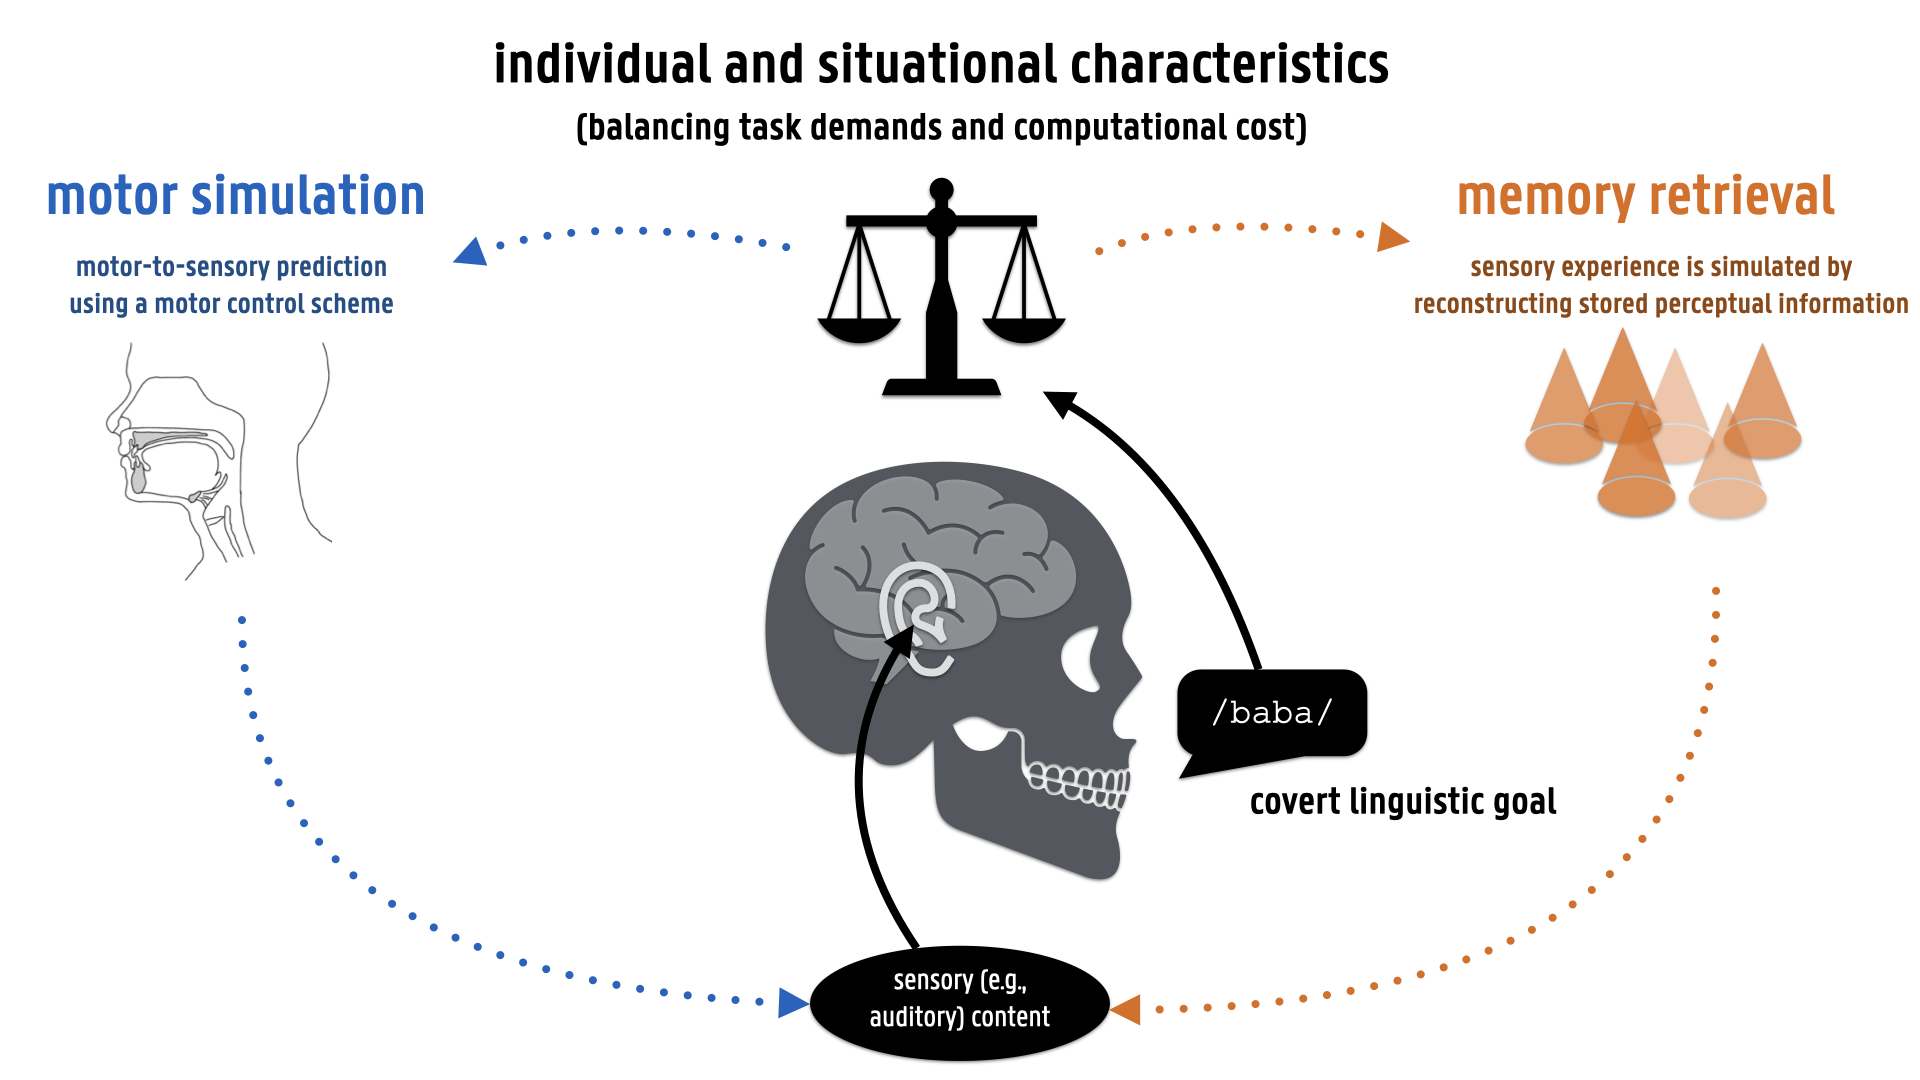
\includegraphics[width=0.75\textwidth]{figures/simulation_association.png} % This is a *.eps file
% \end{center}
% \caption{High-level depiction of the prediction-by-simulation (in blue) and prediction-by-association (in orange) mechanisms. The balance (weighting) between these two mechanisms during covert verbal actions depends on both task demands and "computational cost" (cf. text for more details), which are jointly determined by internal (individual) and external (situational) characteristics (e.g., expertise or (equivalently) task difficulty, noise, feedback perturbation).}\label{fig:1}
% \end{figure}

\begin{figure}[ht] % float was h! initially
\begin{center}
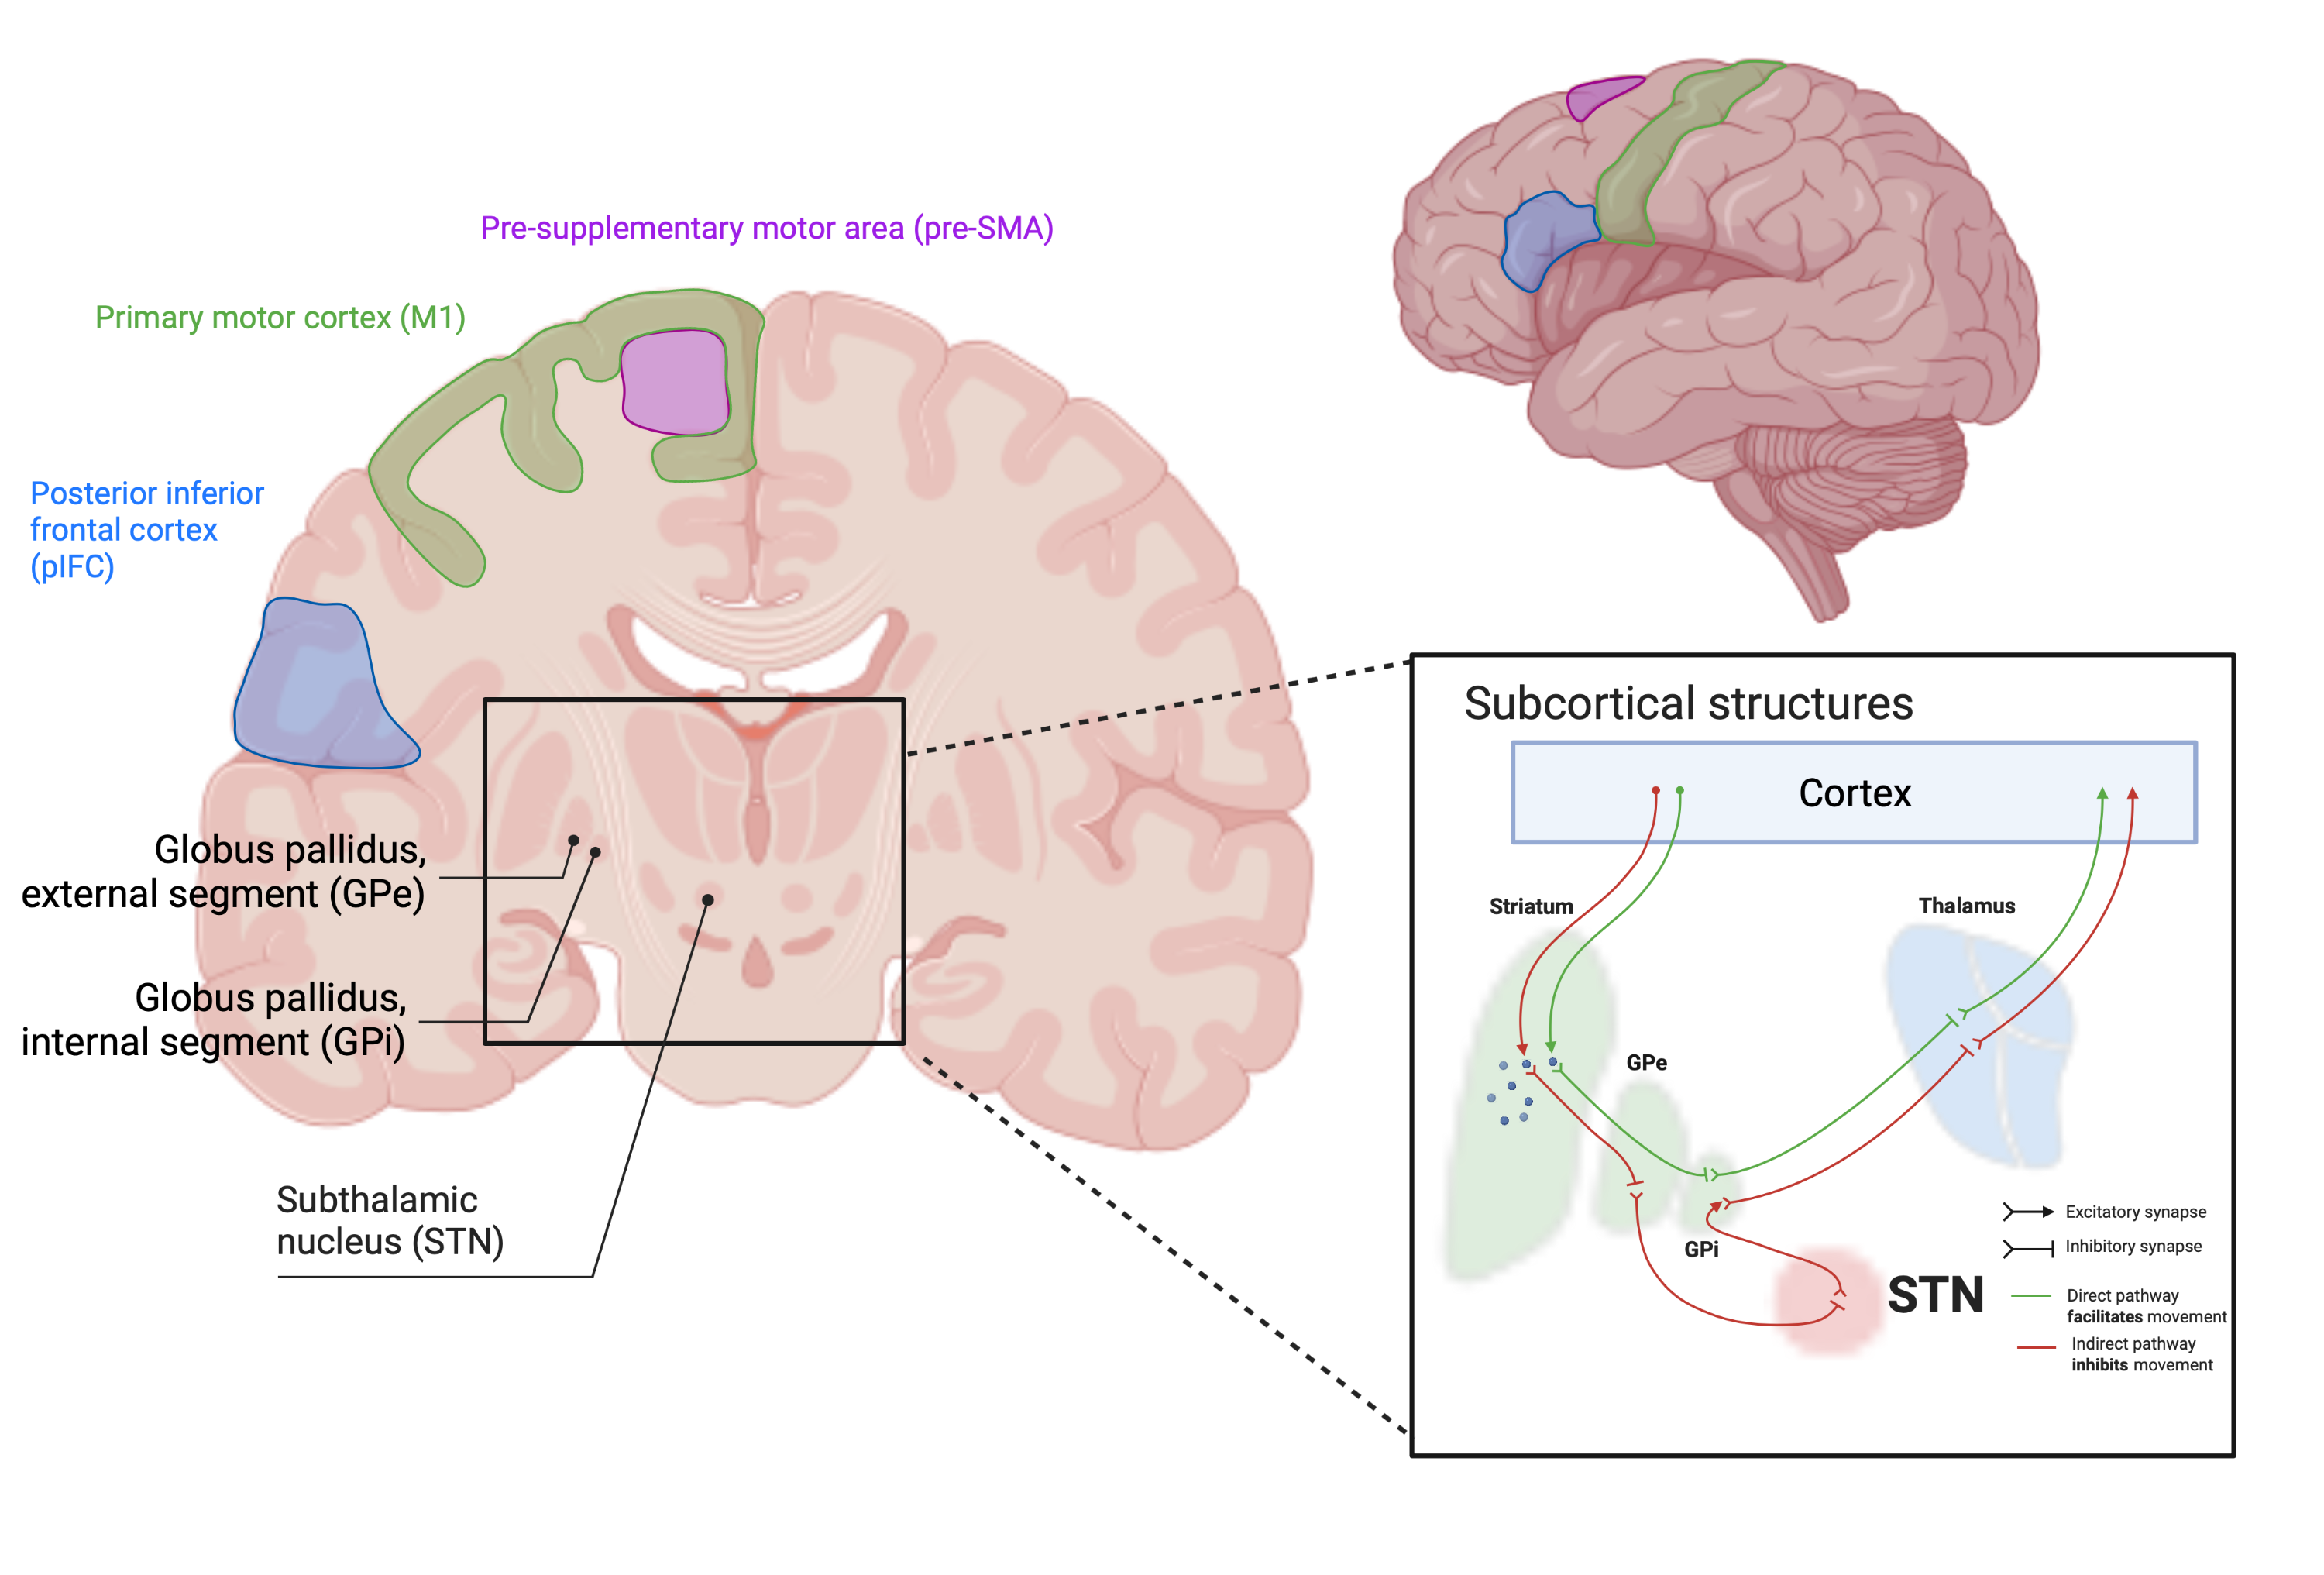
\includegraphics[width=0.75\textwidth]{figures/inhibitory_triangle.png} % This is a *.eps file
\end{center}
\caption{Plausible neural implementation of the (cortical and subcortical) inhibitory mechanisms responsible for the "proactive" (but implicit) response inhibition at play during motor imagery. The preSMA, right pIFC, and STN together form an \textit{inhibitory network} known as the \textit{inhibitory triangle}, which may be responsible for braking motor commands during covert speech production. Figure created with BioRender.com. FIGURE IN PROGRESS.}\label{fig:2}
\end{figure}

%%% If you are submitting a figure with subfigures please combine these into one image file with part labels integrated.
%%% If you don't add the figures in the LaTeX files, please upload them when submitting the article.
%%% Frontiers will add the figures at the end of the provisional pdf automatically
%%% The use of LaTeX coding to draw Diagrams/Figures/Structures should be avoided. They should be external callouts including graphics.

\end{document}
